%************************************************
\chapter{Literature Review}\label{ch:litreview}
%************************************************
This literature review will first address the current state of data integration within the rail domain, before moving on to addresses the benefits of improved data integration and the means of improving integration. After presenting linked data and ontology as a solution, other industries which have adopted ontology for data integration will be examined and applicable lessons drawn. These lessons will then be applied to the rail industry.

\section{State of the Industry}
\label{state}
The most recent discussion of the state of data integration, \cite{RSSB2017}, published by the Railway Safety and Standards Board, here on referred to as the RSSB, and also discussed in \autoref{ch:intro} does not go into detail as to the current state of rail data integration; rather it expresses aspirations as to how it would like data integration to be in the future. That ``Standards will allow information to be interpreted and combined more easily delivering new insights and intelligence to the industry.'' remains an aspiration, however goes some way to explaining the outstanding work.

Another source of information as to the current state of the railways is the Mc Nulty report \cite{DepartmentforTransport2011}, which has the following to say regarding the railway's information systems (IS) ``The Study has found that the effectiveness of the industry’s IS is inhibited by a suite of legacy systems that are expensive to run, unable to communicate with new technology and encourage users to develop a wide range of bespoke local systems to overcome limitations. Many legacy systems were created and managed in company silos, with only a few systems crossing industry boundaries.''. It goes on to conclude: ``Information systems are at the heart of a more efficient railway that delivers value for money. Allowing the railway’s existing IS to continue unreconstructed will increase cost, reduce efficiency and undermine customer service. In contrast, the replacement of legacy systems and the exploitation of new technology will generate improved value for money.''.  That lock in to proprietary systems and the creation of data silos is a point repeated in: \cite{Joh13}, which states that ``Where electronic data exchange standards for rail do exist, many are proprietary binary formats used to provide point-to-point interfaces between specific systems and not intended for use in a generalised context.''. Verstichel et al in \cite{Verstichel2011a} also find a need for improved data integration in the European  Rail Domain: ``Industry-wide integration in the information domain is only in its infancy. From an efficiency point of view, this field leaves much room for improvement (as did the integration in the mechanical and electrical domain).''

The Rail Technical Strategy \cite{TechnicalStrategyLeadershipGroup2012b}, also identifies a need for better data integration, stating that there are ``over 130 information systems maintained by approximately 20 suppliers were in operation in 2011. Maintaining individual legacy systems is expensive and inefficient. Information cannot be shared or exploited efficiently and this inhibits whole-system approaches for technology-based improvements.''. Much of this work is reported in \cite{Morris2014}, which also reports rising rail rider ship in the UK. This trend continues as shown by the official statistics from the Office of Road and Rail, \cite{OfficeofRoad&Rail2016}, with 1.7 billion journeys having been made in the financial year 2016-17, up 0.8\% from the previous finical year, which marks the highest ever number of journeys on the UK rail network, since statistics started being collected in 1950. It should however be noted that this is the smallest year on year increase since 2009-10.

The amount of data used within the rail domain has increased steadily with time. As it has become possible to collect more data on asset condition for example then the volumes of data relating to each asset have grown. An assessment of the growing volume of data in the rail domain, in an American context may be found in: \cite{Zarembski}. Similar challenges are faced in the European Rail Domain, with techniques such as alternating current field measurement sensor (ACFM) as discussed in \cite{Rowshandel2013}. The growing volumes of data handled by the European rail network are addressed in \cite{Nunez2014} which also studies data used for maintenance in the rail domain, taking as a case study the Dutch Rail Network.  In the UK large volumes of valuable data are collected by the New Measurement Train. Another source of high volumes of data is ground penetrating radar, to assess trackbed condition, as reported in: \cite{eriksen2004improved}.

The current work flow with regards wheel impact load detection, which was described in \cite{Tutcher2015} as: ``several interfaces between machine and human operator railway data management,  exist, as wheel impact data is taken from its silo, manually compared to train running information in another silo, and finally input into a maintenance system silo''. Wheel impact load is important because it detects when train wheels are damaged, thus in turn causing damage to the track and train alongside causing discomfort to passengers.

Another issue addressed in this thesis is that of IT security in the rail domain the importance of which is discussed in \cite{Depar2016}. A discussion of the cyber security of signalling systems may additionally be found in: \cite{BloomField2016}.

\section{benefits}
\label{benefits}

Many of the same reports and paper as discuss the currently poor integration go on to discuss the expected benefits of data integration. In \cite{RSSB2017} the most important benefit considered is the cost reduction, similarly \cite{Verstichel2011a} looks at the efficiency improvements. 

Another benefit of better data integration, discussed in \cite{Tutcher2013} is as an enabler of other improvements, in this case remote condition monitoring. Passenger information is another commonly cited beneficiary of ontology \cite{Verstichel2014}. The TraPIST project discussed in \cite{Verstichel2014} implements a framework for data integration using ontologies and creates a real time passenger information application as a demonstration. A network statement checker was also produced, as reported in \cite{Verstichel2011a} which is another application of ontology in the rail domain.

The advantages to the rail domain of using ontology are discussed in \cite{Morris} based on discussions with the UK infrastructure manager, Network Rail, as well the study reported in: \cite{Roberts2011}. The use cases examined in that study were:
\begin{description}
    \item[Customer Information] This is discussed in many studies, including the possibility of going beyond simply informing the customer of the time table and when a particular train is expected, to outlining possibly connections in light of real time information as discussed in \cite{Verstichel2014}. 
    \item[Predictive maintenance]
    This is an area in which Ontology acts as an enabler, rather than being used directly; much work exists in the area of predictive maintenance, but it is only possible when data is available. The project, reported in \cite{Tutcher2015a} addressed this issue and produced a demonstrator looking at points machine condition monitoring. This is discussed further in \cite{Umiliacchi2011}.
    \item[Train Identification]
    The linking of track-side information with running services is discussed in \cite{Morris}. Condition monitoring of in service vehicles from the track-side currently presents challenges linking the vehicle detected to a physical unit is a problem. 
    \item[Maintenance Timing and Forward Planning]
    Two scenarios put forward by the UK infrastructure manager, Network Rail, revolved around forward looking question answering. An interface should be provided to allow the asking of guided (not truly free text) questions such as: ``Given the data we have when would be the best time to do maintenance?'' or ``Is it better to replace a given asset, such as a bridge, like for like or with a less expensive substitute, such as a bridge rated for a lower weight?''    
\end{description}

Several European Projects, recently IT2Rail as reported in \cite{Gogos2016}, discuss the advantages of using ontology for data integration in the rail domain. As with previous studies, such as InteGRail, reported in \cite{Kopf2010}, they find it to brings benefits to the domain as a whole, even where such benefits do not accrue with the same party as the costs. A key advantage of using ontology for data integration, as espoused by \cite{Gogos2016} and \cite{Morris}, is that of decentralising data entry. By defining a standard which can be extended by anyone there is no limit on who can make data available to the domain. Furthermore the architecture of semantic web means that there is no need for a central repository of all rail related data; rather it is possible for suppliers to host data on there own products and for this to be available as needed. Security restrictions may be placed on who can access certain data when that is necessary.

There several currently running European Projects building upon IT2Rail for passenger information notably the `Co-Active' and `ATTRACkTIVE' projects with in the shift to rail framework, though these have yet to publish. Ontology can bring a range of benefits to the customer information domain, integrating data from various sources to provide more comprehensive information. The work reported in \cite{Verstichel2014} included a customer assistance application, which aimed to give personalised customer information for users making multi-modal journeys. The framework developed to support this is discussed later in this chapter. Using data from multiple sources, both timetable and actual running, along with GPS position and personalisation setting, such as the user mobility the application will attempt to suggest the best modes of transport to complete a journey, according to the users selected metric (cost or time). 

\section{Multi-modal transport}

Multi-modal transport is a domain in which by very definition there is a strong need for data interchange. Real life journey's tend to be multi-modal and thus it is beneficial for journey planning applications to include multiple modes. The work in \cite{Verstichel2014} reflects that, however this was first considered in the ArkTRANS project, as reported in various papers including \cite{Natvig2003}. This is further reviewed in \cite{Morris2016}, which goes on to discuss Google Transit Feed Specification, here on refereed to as GTFS. GTFS is discussed in \cite{Santos2014} and it's success should be noted; much public transport information is now available to google maps. Possible improvements to the protocol are discussed in \cite{Santos2014} and further improvements have been proposed by google, in particular to allow real time information to be added to the map, regarding departures and service status. The original GTFS defined at: \url{https://developers.google.com/transit/}. It can be seen that GTFS is a fairly simple relational format. It is heavily used, as described in \cite{Colpaert} ``The General Transit Feed Specification (GTFS)3 specifies the headers of 13 types of CSV files, describing the schedules using a set of rules. In recent years, GTFS gained a lot of popularity, thanks to its simplicity and its adoption in popular route planning systems such as Open Trip Planner, Navita.io, Google Maps or RRRR Rapid Real-time Routing.'' The work in \cite{Colpaert} uses GTFS and linked data fragments to perform multi-modal route planning.

Multi-modal transport of freight is also considered; \cite{Gonczy2012} in particular looks at this, though it was previously considered as part of the ArkTRANS project. Freight transport, like passenger, is often multi-modal though the modes differ, notably other parts of the ArkTRANS project, notably \cite{Rødseth2011}, touch on sea freight. Another, project to investigate the use of ontology in freight is \cite{Paganelli2009}.

\section{Work done in other industries}
It should be noted that many other industries are far ahead of the rail industry in terms of take up of ontology. In \cite{Morris2014} the following industries are discussed:

\begin{description}
	\item[Bio-Medical Research]  
	The Bio-medical domain was at the forefront of uptake of ontology. \cite{Grenon2004} suggested design principles for a biomedical ontology, in particular it proposed using Basic Formal Ontology (a high level ontology) as a basis for a biomedical ontology and discusses the principles behind BFO. As early as 2004 the Gene Ontology (GO) was available for use and was described as by \cite{Smith2004} as ``As of March 15, 2004 GO comprehends 1395 component terms, 7291 function terms, and 8479 process terms. These form three separate graphs, whose primary purpose is to allow researchers annotating genes and gene products to locate where the features and attributes they are addressing in their work might lie (their position in logical space) in relation to other, more familiar features and attributes and thus either to pick out corresponding terms already existing within GO’s controlled vocabulary or to localize corresponding gaps in the existing hierarchies and so recommend new terms which need to be included.'' In 2006 \cite{Bodenreider2006} summarised the the role of ontologies within bioinformatics as as having ``moved from a niche activity to one that is, in all respects, a mainstream activity''. That study includes a time line, until 2006 (when it is published) of use of ontology within bioinformatics, which shows a move from ontologies designed by computer scientists to ontologies produced within the bioinformatics community. Discussing specifically the Gene Ontology \cite{Bodenreider2006} states that it grew from 3500 terms in 1998 to 20,000 terms in 2006. It is worth noting that both \cite{Bodenreider2006} and \cite{Gro2016} as with other studies in the domain of bioinformatics are careful to state that they are defining ontology quite broadly; there is room for argument, though it is beyond the scope of this thesis, as to whether these some of the ontologies in this domain might more properly be termed ``controlled vocabularies''. A recent study, \cite{Gro2016} focuses on mapping the various related ontologies in the bioinformatics domain together and studying how they change. It finds 500 different ontologies to be in use at this time in bioinformatics.
    \item[Media]    
    The British Broadcasting Corporation, here on refereed to as the BBC make extensive use of ontology, both internally and externally\footnote{A promotional video  for the BBC's work in this area may be found at: \url{http://www.bbc.co.uk/academy/technology/software-engineering/semantic-web/article/art20130724121658626}}. The BBC also adopted linked data comparatively early; \cite{Geo09} talks not only about the BBCs aspirations and future plans but about progress already made and says: ``we demonstrated how these links between data items can benefit our user facing web sites, through topic pages and navigation badges.'' It is worth noting that the BBC made use of several external data-stores, most notable amongst them DBPedia - \url{http://wiki.dbpedia.org/}, a linked data companion to wikipedia. As discussed in \cite{Mikroyannidi2016} the BBC have continued to make progress in this area, now covering the education domain.  
    \item[Process and petrochemical plant] ISO15926 was published in 2004. \footnote{Defined at: \url(https://www.iso.org/standard/29556.html}. This in turn grew out of a standard for exchanging CAD drawings. A history of ISO15962 is available at: \url{https://www.posccaesar.org/wiki/ISO15926Primer_ShortHistory}. In particular this standard has been used by oil companies working on the ``Norwegian Continental Shelf''. As discussed in \cite{Leal2005} The standard's key components are a reference data model and an information model. The concepts used in ISO15926 and in particular it's approach to modeling how things change over time where important in informing the design of the rail core ontologies, as discussed in \cite{Tutcher2015}, along with a more detailing break done of the standards components. 
    \item[Power Distribution] The common information model, as used in the power distribution industry is extended in \cite{Hargreaves2013} to include use of ontology for information exchange.
\end{description}
There is on going work in several domains, at various levels of maturity.
\begin{description}  
	 \item[Manufacturing]
	the work covered by ISO15926 \cite{Mueller2015} proposes ontology as a means to reduced energy consumption. A generic manufacturing ontology was produced by \cite{Mazzola2016} under the auspices of the Horizon2020 program.
    \item[to do]
    Furthermore recently other sectors have started using linked data, notably geospatial data {just list everyone who went to KEOD}
\end{description}

\section{Previous Work}
\subsection{Non-ontology data integration}
Data integration has been required within the rail domain for longer than ontologies have been used within the software domain. As such standards were developed for data interchange on an as required basis, whenever two or more systems to communicate. Many of these have evolved over time and have value in different domains. The key weakness with all such approaches is there inflexibility; when the information to be exchanged changes so must the standard, such interfaces are however generally computationally in expensive to implement. A good a assessment of the currently used data interchange standards may be found in \cite{Tutcher2015} Chapter 3, which covers the following systems and interfaces:
\begin{description}
    \item[DARWIN] Is the current UK solution for providing real time passenger information, pulling together train describer information with information from various operating company specific systems which offer better precision. This is then made available both to station displays and to external users via web-services.
    \item[ORBIS] Offering Rail Better Information Services (ORBIS) is described in \cite{Tutcher2015}  as ``a series of projects centred around providing staff with better access to existing asset information data''
\end{description}



\subsection{Prevous ontologies based integration}
Previous studies have examined ontology in the rail domain and in particular developing data models covering the rail domain. Other studies, notably the TraPIST project as most recently reported in \cite{Bhatti2016} have explored making ontologies usable by industry, though in that case the emphasise was on customer information. This study is interested in covering the domain for any purpose; the demonstrators produced centre on signalling and past projects have been centred around condition monitoring.

Before any work was done specifically on the rail domain specifically there where other more general ontologies which touched on the transport domain. These are neither intended for, nor possible to use as, a means of integrating data within the rail domain, however, by taking an upper ontology as the basis for a domain ontology it makes integrating multiple domain ontologies easier. The Suggested Upper Merged Ontology (SUMO) proposed in \cite{Niles2001} is an example of such an upper ontology which has very high level coverage of the rail domain.

 The REWERSE project reported in \cite{Lorenz2005a}, part of the Sixth Framework Program, also produced an ontology which covered the transport domain. The purpose of this project was primarily the interchange of geographic information, however transport modes are covered in some depth, including interchanges between modes and routes taken. Further, beyond the mapping domain this ontology allows for the modelling of timetables for all modes of transport. Road transport and  restrictions such as speed, class of vehicle etc are also modelled. Whilst the goal of this project was not to provide an ontology suitable for detailed evaluation of vehicles or fixed assets within the rail domain it could be applied to the integration of multi-modal transport.

The InteGRail project reported in \cite{Kopf2010} was a European project also funded as part of the Sixth Framework Programme. This aimed to produce both an architecture and an ontology for data integration, to act as a standard for data interchange within Europe. The demonstrator produced at the end of this project was a ``network statement checker'', this tool allowed users to check if a given train consist was compatible with a chosen route. The work done as part of InteGRail is discussed further in \cite{Verstichel2011}, as is the importance of adding semantics to data for improved integration. In particular the the InteGRail project makes possible integration not just of data from different manufacturers but also different countries - where trains are to run across boarders there is a more significant data integration challenge. At the simplest level it is easier to ascertain whether a track is of the same width, or gauge, as the proposed train consist. Other details are less striate forward; the required characteristics of the electrical supply in terms of voltage frequency and current must be correct, as must the means of ``picking up'' the power - overhead line or third rail. More complex issues are presented by the loading gauge (other physical aspects of the vehicles, which determine whether they can clear corners, bridges, platforms etc.) and signalling or train control system used, which as  more complex systems are developed because more problematic, though standardisations efforts in this domain are well under way. As discussed in \cite{Verstichel2011} Ontology can handle such relationships as one train control or signalling system being a subset of or synonyms for another, relationships which would at best need to be specifically planned for if used a pre-defined schema, such as is found in a relational database.

The work on which this most directly thesis most directly builds upon is that done at this centre and reported in \cite{Tutcher2015}. This study centred around the principles of designing ontologies for the rail domain. The result was the Rail Core Ontologies, refereed to by the author as RaCoOn, a group of ontologies for representing the rail domain in depth and a set of design principles for extending them as necessary. This resulted in a group of ontologies arranged as in \autoref{fig:RacoonLayers}. Note the hierarchical arrangement of the layers. The highest layer, the upper ontologies, contain concepts which apply outside of the rail domain. It is this layer which could be mapped to concepts in an external upper level ontology where integration beyond the rail domain required. In \cite{Tutcher2015} DOLCE Utlra-Lite and The Basic Formal Ontology (as discussed in the context of Bio-Sciences) are considered.

\begin{figure}[htb]
\myfloatalign
{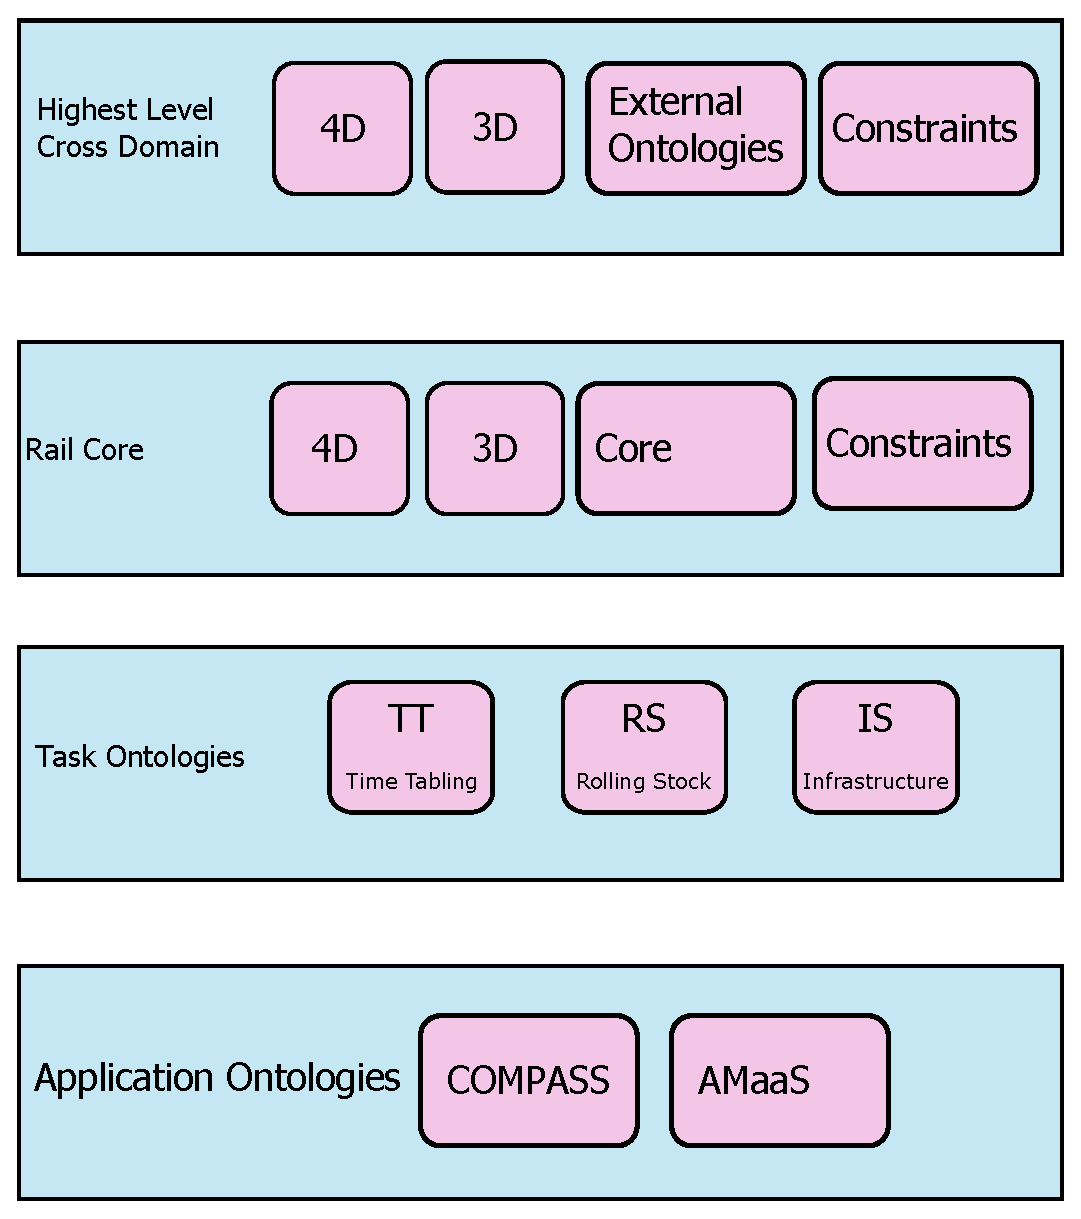
\includegraphics[width=0.6\linewidth,keepaspectratio]{gfx/RacoonLayers}} 
\caption[Racoon Layers]{Structure of the RaCoOn Ontologies}
\label{fig:RacoonLayers}
\end{figure}

In line with with



